\scanpage{79}
% archive foliation: 78
fait $H^1(\mathbf{F}_p,A^{\mathrm{fix}})=0$ (Lang) et $H^1(\mathbf{F}_p,M)=\text{fini}$ [\unsure{triv.|trivial} ; Attention qu'il s'agit de la coh. \uline{étale}, i.e. de la coh. \uline{galoisienne} de $\widehat{\mathbf{Z}}$ !], donc la dernière flèche verticale du diagramme (\unsure{D|b}) est aussi bijective :
\[
H^1(S,A)(\ell)\xrightarrow{\sim}H^1(\overline{S},\overline{A})^\pi(\ell)
\]
\margin{\uline{surj. à noyau fini} ...}
Donc la \uline{conjecture} précédente signifie aussi
\[
\boxed{H^1(\overline{S},\overline{A})(\ell)^\pi=\text{groupe fini}}
\]

\deleted{Il y a une façon de le prouver,}
C'est \inserted{aussi} $\pm$ équiv. (via des jacobiennes) à ceci : $X\unsure{-|\longrightarrow}S$ morphisme propre [lisse de dim relative $1$], $S$ régulier de type fini sur $\mathbf{Z}$. Prouver que
\[
H^2(S,\mathbf{G}_m)\longrightarrow H^2(X,\mathbf{G}_m)
\]
est surjectif mod groupes finis ??
\figure{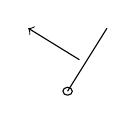
\begin{tikzpicture}[x=1mm,y=1mm]\draw (0,0) ellipse(.6mm and .5mm);\draw (0,0)--(5,8);\draw[->] (1.5,4)--(-5,8);\end{tikzpicture}}

\margin{\uline{NB} On devrait avoir $H^{\unsure{2|i}}(S,A)(\ell)$ fini aussi pour $\uuline{i\ge3}$, $S$ de type fini sur $\mathbf{Z}$, $\ell$ premier avec \unsure{car.} visiblement \unsure{on} (\inserted{\uline{NB}} si $i\ge2$, $T_\ell(H^i(S,A)(\ell))\simeq H^i(S,T_\ell(A))$)}
\margin{\unsure{donc les seuls} \illegible{1} \unsure{qui restent} sont $H^0$ et $H^2$ pour $A$, et \deleted{$\unsure{H^0}$}, $H^1$, $H^2$ pour $T_\ell(A)$}
